In this section, we present a novel method for approximating piecewise linear functions. The goal of this algorithm is to reduce the number of partitions of a piecewise linear function represented in case form. This represents the ability to automatically identify and remove locally unimportant constraints, whose removal results in a small change in the represented function in exchange for a significant improvement in the efficiency of computations with these functions. XADDs already permit compactness by exploring variable and context independencies, so our approximate approach goes further to merge partitions as a form of removing dependencies that had little influence in the represented function.

\subsection{ Linear Approximation by Successive Merging}
It is important to note that our merging strategy involves calculating a new case linear function, that can optimally approximate the two previous linear cases but be of a reasonably distinct kind, for instance it may not be obtainable as a linear combination of the original case functions. 

In general, however, it isn't clear how a best linear approximation for various partitions can be directly constructed. Thus, our approximation algorithm~\ref{alg:approx} uses a constructive strategy to obtain merging of arbitrary regions by successive pairwise merging of linear case functions. This idea is simple and is illustrated in figure~\ref{fig:steplining}. The bounded error property comes from keeping the amount of error "used" in every merge and avoiding any merges that incur more error than the remaining allowed error on one of the nodes being currently merged.

\begin{figure}[!ht]
\centering
  \subfigure[Original] {
	\fbox{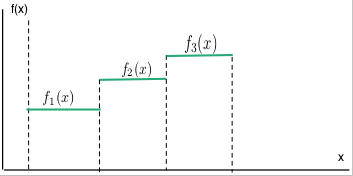
\includegraphics[width=.3\textwidth]{Figures/stepfun/step1.png}}
	\label{original}
  }

\subfigure[Step1] {
	 \fbox{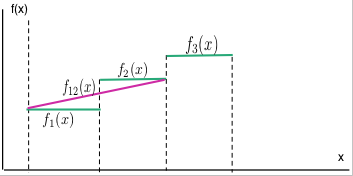
\includegraphics[width=.3\textwidth]{Figures/stepfun/step12.png}}
	\label{step1} 
}

\subfigure[Step2]{
	 \fbox{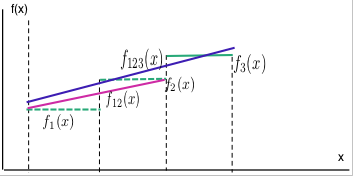
\includegraphics[width=.3\textwidth]{Figures/stepfun/step123.png}}
	 \label{step2}
}

\caption{ Approximation by successive pair merging}
 \label{fig:steplining}
\end{figure}

\begin{algorithm}[!ht]
\dontprintsemicolon
\KwIn{A piecewise linear functions $V$, allow\_error}
\KwOut{Approximated version of $V$.}
$OpenCases \gets getCases(V)$\;
\While{$OpenCases != \emptyset$} {
	$L_1 = OpenCases.pop()$\;
	$error = allow\_error$\;
	\For{$ L_2 \in OpenCase$}  { 
		$MergeResult = PairwiseCaseMax( L_1, L_2)$\;
		\If {$ MergeResult.error < error $} 
		{
			$error \gets error - MergeResult.error$\;
			$OpenCases.remove(L_2)$\;
			$ Remap(L_1, MergeResult.L^*) $\;
			$ Remap(L_2, MergeResult.L^*) $\;
			$ L_1 \gets MergeResult.L^* $\;
		}
	}
}
\Return{ApplyRemap(V)}\;
\caption{{\sc Approximate} bounded error approximation of a symbolic function by successive case merging}
\label{alg:approx}
\end{algorithm}

\subsection{ Optimal merging of linear case functions}

In the last section we have shown that the the general piecewise linear approximation may be reduced to the smaller, pairwise case linear function approximation. Our main contribution in this paper is the development of an iterative linear program based algorithm for obtaining optimal, that is, max-error minimizing, case linear functions for any pair of case linear functions. In order to explain our algorithm more conveniently, we make some clarifications on denotation and simplification.

First, since the continuous domain of a case linear function is independent of boolean variables, they do not interfere with the maximization of the linear functions and therefore don't change the merging of linear case functions. Our approximation works independent of the boolean variables, so we will consider piecewise linear functions whose partitions are defined only with linear inequalities. We observe that regions defined by conjunctions of linear inequalities are (possibly unbounded) polytopes and a disjunction of such formulae is the union of the  regions defined by each sub formula, so that a generic formula $\phi$ of linear inequalities is equivalent to a region  $S(\phi)$ defined by a union of polytopes $\theta$. We denominate $Poly(\phi)$ the set of all polytopes generated expanding disjunctions of $\phi$.

Second, since we are only representing linear functions, all functions $f$ must be of the form 
$f(\vec{x}) = \vec{c}\cdot \vec{x}_0$ , where $\vec{x}_0$ denotes the extended vector 
$(1,\vec{x})$ to include the constant term $c_0$ of $f$. This means that the domain of linear function on $\vec{x}$ is isomorph to $\mathbb{R}^{m+1}$. We call elements of this space parameter vectors $\vec{c}$.
We can now proceed to defining the crucial step for the approximation algorithm, modeling optimal merging of linear case functions as an optimization problem.

More formally, given two case linear functions $L_1 = ( f_1, \phi_1 )$ and $L_2 = ( f_2, \phi_2 )$, our goal is to determine the best linear case approximation of $L_1$ and $L_2$. As it must represent  $L_1$ and $L_2$, the solution must be defined in both regions, therefore of the form $L^* = (f^*,\phi_1 \lor  \phi_2)$ . In this case, we must find a linear function $f^*$ that minimizes approximation error $E$, defined as the maximum  error of replacing both $f_1$ in $\phi_1$ and $f_2$ in $\phi_2$ by $f^*$:

\begin{equation} E(f) = \max ( |f - f_1|_{\phi_1} , |f - f_2|_{\phi_2} ) \label{maxphase} \end{equation}
\begin{equation} f^* = \argmin_f E(f)  \label{minphase} \end{equation}

Note that the absolute value in~\ref{maxphase} is equivalent to max of two linear functions, e.g. $|f - f_1| = max ( f - f_1, f_1 - f)$. Moreover, each of these partition $\phi_i$ constrained max is equivalent to the max in all polytopes $\theta_{1{i_1}}$ of $\phi_i$. With this, we can rewrite the error $E$ as the maximum of a finite number of errors restricted to polytopes, e.g.:
{\footnotesize 
\begin{align}
 e_{1{i_1}}(f) &= max_{\vec{x} \in \theta_{1{i_1}}} (f - f_1)(\vec{x}) \forall \theta_{1{i_1}} \in Poly(\phi_1) \nonumber\\
 e_{2{i_2}}(f) &= max_{\vec{x} \in \theta_{2{i_2}}} (f - f_2)(\vec{x}) \forall \theta_{2{i_2}} \in Poly(\phi_2) \nonumber\\
 e_{1{i_3}}(f) &= max_{\vec{x} \in \theta_{1{i_3}}} (f_1 - f)(\vec{x}) \forall \theta_{1{i_3}} \in Poly(\phi_1) \nonumber\\
 e_{2{i_4}}(f) &= max_{\vec{x} \in \theta_{2{i_4}}} (f_2 - f)(\vec{x}) \forall \theta_{2{i_4}} \in Poly(\phi_2)\nonumber\\
E(f) &= max_{k=1..K} (e_k(f)) \nonumber
\end{align}
where $K$ is the total number of pairs (linear function, polytope)  and e$ _k$ is an enumeration of all $e_{nj}, n = 1,2; j $ is index of a polytope.
}

This is a complex bilinear piecewise optimization problem, involving minimization on the parameters $\vec{c}$, maximization on the original continuous variables $\vec{x}$ and case max between the polytope maximums, thus we can break it down to a three step optimization problem: 

(i) There are linear constrained bilinear functions $L_{k}(f,\vec{x},\phi_k) =  ( l_k(\vec{c},\vec{x}) ,\phi_k)$ depending on both the domain variables $\vec{x}$ and parameter variables $\vec{c}$, defined in $\phi_k$ such as $ ( (f - f_1)(\vec{x}),\phi_1) = ( (\vec{c}-\vec{c_1})\cdot\vec{x}, \phi_1)$. The innermost optimization step is the constrained maximization of this bilinear function on the domain variables.
\begin{equation} e_k(f) = max_{\vec{x}} ( L_k(f,\vec{x},\phi_k) ) = max_{ {\vec{x}} \in \phi_k} (l_k (\vec{c}, \vec{x}) ) \label{optim1} \nonumber \end{equation}

(ii)There is a case max in a finite group of this linear constrained bilinear functions :
\begin{equation} E(f) = \max_{k=1..K} ( max_{\vec{x}} ( L_k(f,\vec{x},\phi_k) )) = \max_{k=1..K} ( e_k(f)) \label{optim2}  \nonumber \end{equation}

(iii)Finally, this case max is minimized in terms of the parameters $\vec{c}$ as in ~\ref{minphase}:

In order to solve it we propose an elaborate iterative constraint generation based algorithm~\ref{alg:glo}, which we describe in the following.
First, the algorithm will iterate between two phases, one for the maximization and one for the minimization.  Second, on each phase a relaxed problem will be solved using the result from the previous phase. Third, when a phase gives the same return twice, the algorithm has converged.

TODO: It would be nice to have a diagram around here (and I can't make one fast ENOUGH)

\begin{algorithm}[!ht]
\dontprintsemicolon
\KwIn{Linear cases  $L_1 = ( f_1, \phi_1 )$, $L_2 = ( f_2, \phi_2 ).$}
\KwOut{ $(L^*, error)$ s.t. $L^*$ approximates $L_1$ and $L_2$.}
$f \gets 0$\;
$points \gets \emptyset$\;
$new\_points, error = MAX\_ERROR(f, L_1,L_2)$\;
\While{$new\_points \not \subset points$} {
	$points = points \cup new\_points$\;
	$f = BEST\_APPROX(f_1,f_2,points)$\;
	$new\_points, error = MAX\_ERROR(f, L_1,L_2)$\;}
\Return{$( (f, \phi_1 \lor \phi_2), error )$}\;
\caption{{\sc PairwiseCaseMax} finds the best case linear function}
\label{alg:glo}
\end{algorithm}


In the maximization phase, related to eq.~\ref{maxphase}, we will always assume a fixed $f$, and thus the maximization of the bilinear functions $L_{k}(f,\vec{x},\phi_k)$ for each linear case function will be a linear constrained linear program, solved efficiently by a LP solver. The optimal values are upper bounds on the actual minimal error in each polytope. More importantly, the vertexes that reach this optimal values are the points of the polytope that maximize the bilinear function for this function $f$ and thus are important points to which the minimization must attempt to reduce the error (in fact reducing the error in any set of points that doesn't contain this point won't change the maximal error, and thus won't improve our solution.

In the minimization phase, we will solve a relaxation of~\ref{minphase}, where in each linear constrained bilinear function $e_k$ the maximal error in the polytope $\theta_k$ is replaced by the greater of the error in a finite set of points. More specifically, we only minimize the greatest of the error on points found in the maximization phase. This changes the piecewise bilinear problem into a linear program with the objective to be minimized is the error, and linear constraints encode that this relaxed error $\tilde{E}(f)$ must be greater than the error on any of the previously obtained points. As shown in the following where $x^k_j$, $j=1..m_k$ are the points found in the polytope $\theta_k$:

$$ \tilde{E}(f) =\max ( L_k (f, x^k_1, \theta_k), ... , L_k ( f, x^k_{m_k}), \theta_k ), k = 1, 2, .. K$$
$$\tilde{f} = argmin_f\tilde{E}(f) = argmin_{f,Z}  Z $$
s.t. 
$$
	\begin{array}{llll}
		Z & \geq & L_1(x^1_j, \theta_1) & \mbox{for } j = 1,...m_1\\
		Z & \geq & L_2(x^2_j, \theta_2) & \mbox{for } j = 1,...m_2\\
		Z & \geq & L_3(x^3_j, \theta_3) & \mbox{for } j = 1,...m_3\\
		\vdots & \vdots & \vdots & \vdots\\
	\end{array}
$$

This is now a linear problem in the coefficients of $f$, the solution Z is the error incurred in the approximation. 
Solving this minimization yields a new solution $f$ whose error is a lower bound on the actual minimal error in each of these points. This can be seen by the following: $f$ may have to be modified to minimize the error in more points in the next iterations, but this can only lead to increasing the error in the points that were present in this iteration. This follows simply form the fact that adding more constraints cannot improve the optimal value of solution for a linear program.


\begin{algorithm}[!ht]
\dontprintsemicolon
\KwIn{Case linear functions $L_1 = ( f_1, \phi_1 ), L_2 = ( f_2, \phi_2 )$ and function $f$ }
\KwOut{Set of points where the error is maximal for each polytope and the optimal $error$.}
$max\_points \gets \emptyset$\;
$error \gets NEG\_INF$\;
\For {$\theta_1 \in Poly(\phi1)$} {
	$sol^+, obj^+ \gets LP\_Solve(max _x, f-f_1,\theta_1) )$\;
	$sol^-, obj^- \gets LP\_Solve(max _x, f_1-f,\theta_1) )$\;
	$max\_points.add(sol^+,sol^-)$\; 	$error \gets max(error, obj^+, obj^-)$\; 
	}
\For {$\theta_2 \in Poly(\phi2)$} {
	$sol^+, obj^+ \gets LP\_Solve(max _x, f-f_2,\theta_2) )$\;
	$sol^-, obj^- \gets LP\_Solve(max _x, f_2-f,\theta_2) )$\;
	$max\_points.add(sol^+,sol^-)$\; 	$error \gets max(error, obj^+, obj^-)$\; 
	}\Return{$(max\_points, error)$}\;
\caption{{\sc MAX\_ERROR} finds the points of maximum error}
\label{alg:maxError}
\end{algorithm}


\begin{algorithm}[!ht]
\dontprintsemicolon
\KwIn{Linear cases $L_1 = ( f_1, \phi_1 ), L_2 = ( f_2, \phi_2 )$ and a set of $points$ where to find the best approximation for}
\KwOut{Best linear case approximation $f$.}
$constr \gets \emptyset$\;
\For {$p \in points$}{ 
	\If {$p \in \phi_1$}{
		$constr \gets constr \cup \{ (Z \geq (f - f_1) (p)), (Z \geq (f_1 - f) (p) )\} $}\;
	\If {$p \in \phi_2$}{
		$constr \gets constr \cup \{ (Z \geq (f - f_2) (p)), (Z \geq (f_2 - f) (p) )\} $}\;
}\;
$f \gets LP\_Solve(min_{f,Z}, Z, constr)$\;	
\Return{$f$}\;
\caption{{\sc BEST\_APPROX} finds the linear function minimizing errors a set of points}
\label{alg:bestApprox}
\end{algorithm}


Finally, we can see why if either of the phases do not produce changes the solution must be optimal for the piecewise bilinear problem as a whole. In the case of the maximization, if all the points generated (in all polytopes) were already in the previous minimization phase than the error in any of these cannot be reduced, and since this points include the points of maximal error in all polytopes the actual global maximal error is achieved in one of them, and therefore no solution can have a better maximal error than the current $f$. Similarly, if a repeated value function $f$ is produced in the minimization this means that this function already minimized the error in its greatest error points (added in the previous maximization) therefore no other function can reduce the error in one of this points and these include the maximal error, se the maximal error cannot be reduced, thus we have an optimal solution.

\subsection{Bounded Approximate SPD}
We will now properly define the Hybrid MDP planing algorithm described in this paper. The SDP algorithm~\ref{alg:vi} was modified from its original exact version by the addition of line \ref{approxline} which calls the algorithm~\ref{alg:approx} which is responsible collecting the cases and making the global approximation by combining the successive pairwise merges. The pairwise merges are solved by the iterative algorithm that uses linear program solvers in the two phases previously defined. The algorithms ~\ref{alg:maxError} and ~\ref{alg:bestApprox} encode the previously defined maximization and minimization phases. Both use an abstract call to a linear programming solver, $LP\_Solve($ max or min$, objective\_function, linear\_constraints)$ which returns the solution and optimal value for the linear program received.




